%-----------------------------------------------------------------
%	ESTRELLES BINÀRIES
%	!TEX root = ./../main.tex
%-----------------------------------------------------------------
\section{Estrelles binàries}
Aproximadament la meitat de les estrelles són sistemes de dos o més components que orbiten en torn a un centre de massa comú. Aquí considerarem només sistemes binaris.

Aquests sistemes es poden classificar segons les seves característiques observacionals. Els diferents grups d'aquesta classificació no són, però, mútuament excloents; així doncs, un sistema binari pot ser a la vegada eclipsant i espectroscòpica.

\subsection{Classificació dels sistemes binaris}
\subsubsection*{Binàries òptiques}
Dues estrelles que jeuen en la mateixa visual no lligades gravitacionalment entre si (ja que estan molt lluny l'una de l'altra), de manera que no formen un autèntic sistema binari.

\subsubsection*{Binàries visuals}
Ambdues estrelles poden resoldre's individualment, i si el període orbital no és molt llarg, és possible seguir el moviment de cadascuna.

Si, a més, la distància al sistema binari és coneguda, la separació entre ambdues estrelles es podrà determinar.

\subsubsection*{Binàries astromètriques}
Si un membre del sistema és molt més brillant que l'altre membre, això no es podrà observar visualment.
\begin{figure}[h]
	\centering
	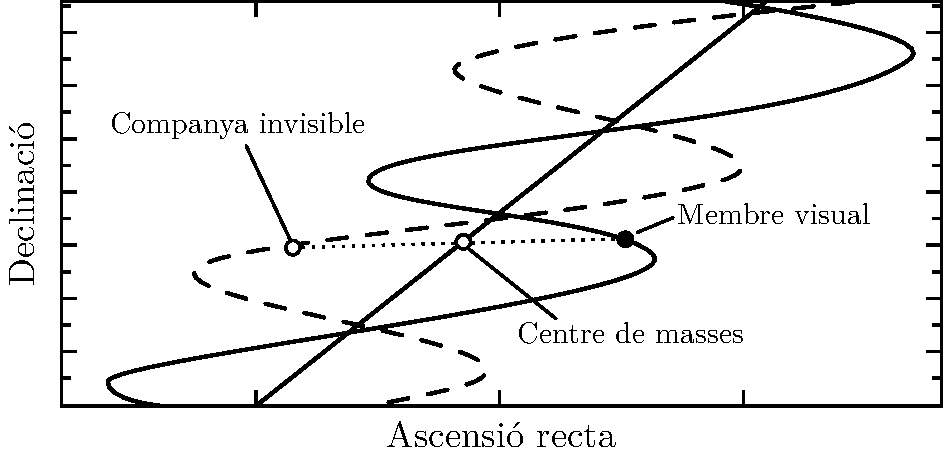
\includegraphics[width=0.7\textwidth]{./images/5-bin-astro}
	\caption{Diagrama de la dinàmica d'un sistema binari astromètric}
	\label{fig:bin-astro}
\end{figure}

No obstant, la seva existència es pot deduir del moviment oscil·latori del primer (figura \ref{fig:bin-astro}).

\subsubsection*{Binàries eclipsants}
Si el pla d'òrbita està orientat aproximadament al llarg de la visual de l'observador terrestre, una estrella passarà periòdicament en front de l'altra interceptant la llum d'aquesta (es produeix un eclipsi).
\begin{figure}[h]
	\centering
	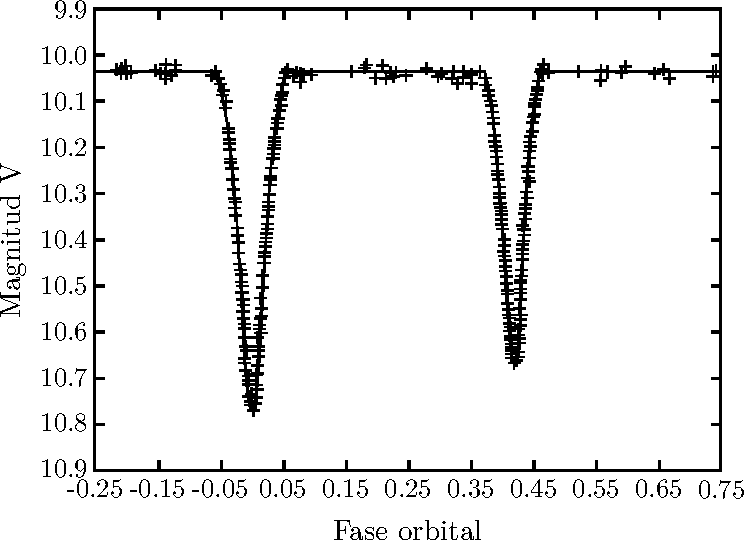
\includegraphics[width=0.7\textwidth]{./images/5-bin-eclip}
	\caption{Corba de llum del sistema YY Sagitari de període \num{2.6284734} dies, excentricitat $\num{0.1573}$, i inclinació orbital $i = \SI{88.89}{\degree}$}
	\label{fig:bin-eclip}
\end{figure}

S'infereix l'existència d'aquests sistemes per la variació periòdica en la llum rebuda al telescopi terrestre (figura \ref{fig:bin-eclip}).

La corresponent corba de la llum proporciona, a més, informació quant al quocient entre les temperatures d'ambdues estrelles, i dels seus radis.

\subsubsection*{Binàries espectrals}
És un sistema amb dos espectres independents, discernibles i superposats. Quan l'espectre d'una estrella està desplaçat cap al vermell, el de l'altra ho està cap al blau i viceversa (respecte de l'espectre que tindrien si es moguessin amb la velocitat constant del centre de masses).

\subsubsection*{Binàries espectroscòpiques}
Si el període del sistema no és molt gran i si el moviment en l'òrbita té una component al llarg de la visual, s'observarà un desplaçament periòdic de les línies espectrals.
\begin{figure}[h]
	\centering
	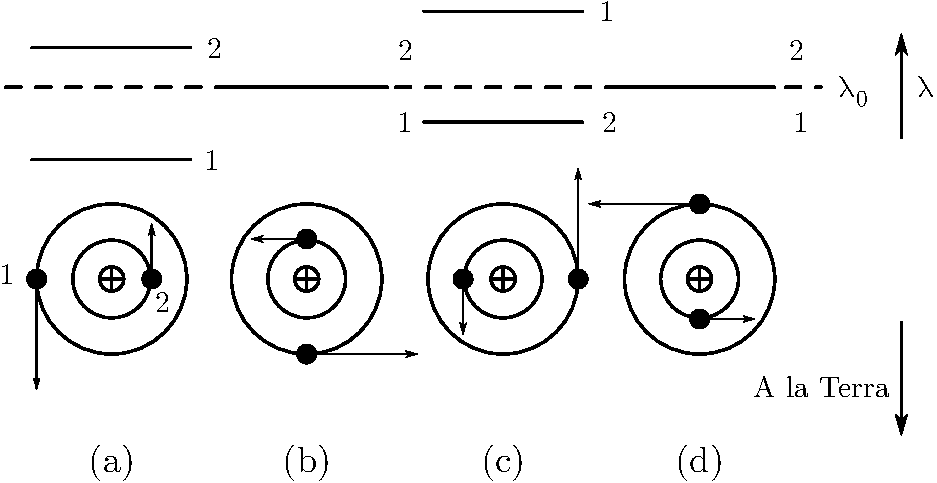
\includegraphics[width=0.8\textwidth]{./images/5-bin-spect}
	\caption{Desplaçament periòdic de les línies espectrals d'un sistema binari espectroscòpic}
	\label{fig:bin-spect}
\end{figure}

Si ambdues estrelles són de lluminositat semblant, ambdós espectres seran observables. No obstant això, si una estrella és molt més lluminosa que l'altra, l'espectre de la menys lluminosa no serà discernible i només seran visibles les línies espectrals de la primera.

Tant en un cas com en l'altre tenim un sistema binari. La figura \ref{fig:bin-spect} il·lustra la relació entre els espectres i les fases orbitals.


%-----------------------------------------------------------------
\subsection{Determinació de les masses d'un sistema binari}
\subsubsection*{Determinació de les masses d'un sistema binari visual}
Aquí ambdues estrelles es distingeixen visualment l'una de l'altra. Prenent l'origen de coordenades al centre de masses ($CM$), tenim
\begin{align}\label{eq:bin-ma}
	\frac{m_{1} \va{r}_{1} + m_{2} \va{r}_{2}}{m_{1} + m_{2}} = \va{0} \Rightarrow \frac{m_{1}}{m_{2}} = \frac{r_{2}}{r_{1}} = \frac{a_{2}}{a_{1}}
\end{align}
on $\norm{\va{r}_{i}} = r_{i} = a_{i}$ és el semieix major de les òrbites el·lipsoïdals de les estrelles.

Els angles subtendits pels semieixos seran (en radiants) $\alpha_{i} = a_{i} / d$, on $d$ és la distància del sistema binari a l'observador. Substituint en l'equació \eqref{eq:bin-ma} es pot determinar el quocient entre les masses:
\begin{align}\label{eq:bin-malpha}
	\frac{m_{1}}{m_{2}} = \frac{\alpha_{2}}{\alpha_{1}}
\end{align}
Les masses individuals també es poden obtenir. Només cal utilitzar l'equació \eqref{eq:bin-malpha} amb la tercera llei de Kepler:
\begin{align}\label{eq:bin-mkepler}
	T^{2} = \frac{4\pi^{2}}{G} \frac{a^{3}}{m_{1} + m_{2}}
\end{align}
on $a = a_{1} + a_{2}$ és el semieix major de l'òrbita de la massa reduïda.

Fins aquí hem suposat que:
\begin{enumerate}[(i)]
	\item El moviment del $CM$ es pot sostreure sense dificultat.
	\item El pla de les òrbites és perpendicular a la visual.
\end{enumerate}
Quan (ii) no es compleix, hi haurà un angle (que anomenarem $i$) entre el pla de les òrbites i el pla del cel (aquest és perpendicular a la visual).
\begin{figure}[h]
	\centering
	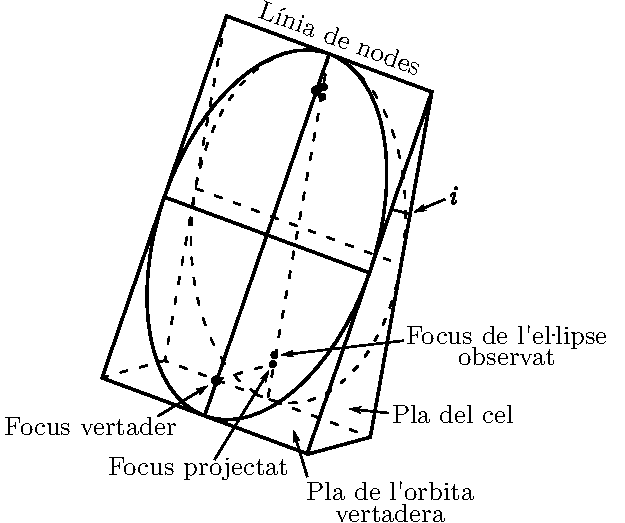
\includegraphics[width=0.6\textwidth]{./images/5-bin-visual-pla}
	\caption{L'òrbita observada és en realitat l'òrbita vertadera projectada sobre el pla del cel}
	\label{fig:bin-visual-pla}
\end{figure}

A la figura \ref{fig:bin-visual-pla} s'ha suposat que la línia de la intersecció d'ambdós plans és paral·lela al semieix menor (cal recordar, de pas, que les òrbites d'ambdues estrelles jeuen sobre el mateix pla).

L'observador terrestre no mesura en realitat $\alpha_{1}$ i $\alpha_{2}$, sinó que la seva projecció sobre el pla del cel: $\tilde{\alpha_{i}} = \alpha_{i} \cos i$. Llavors, en comptes de l'equació \eqref{eq:bin-malpha}, tenim la seva equivalent
\begin{align}
	\frac{m_{1}}{m_{2}} = \frac{\tilde{\alpha}_{2}}{\tilde{\alpha}_{1}}
\end{align}
Tenint en compte que
\begin{align*}
	a = \alpha d = \frac{\tilde{\alpha}}{\cos i} d
\end{align*}
on $\tilde{\alpha} = \tilde{\alpha}_{1} + \tilde{\alpha}_{2}$, en comptes de l'equació \eqref{eq:bin-mkepler} ara tenim
\begin{align}
	T^{2} = \frac{4\pi^{2}}{G} \frac{(\tilde{\alpha}/\cos i)^{3}}{m_{1} + m_{2}} d^{3}
\end{align}
Veiem, doncs, que l'angle $i$ efectivament intervé en la determinació de les masses, i aquest s'ha d'obtenir esbrinant la posició aparent del $CM$ sobre el pla del cel.

Fins i tot en el cas en què la distància $d$ al sistema binari sigui desconeguda és possible trobar $m_{1}$ i $m_{2}$. Per això es necessita conèixer la projecció dels vectors velocitat d'ambdues estrelles sobre la visual. Això, juntament amb la informació quant a les posicions de les estrelles i l'orientació de les seves òrbites, permet esbrinar els semieixos majors d'ambdues òrbites.

%-----------------------------
\subsubsection*{Determinació de les masses d'un sistema espectroscòpic binari}
En aquest cas tenim desplaçaments Doppler periòdics de les línies espectrals d'ambdós components del sistema.
\begin{itemize}
	\item Si les òrbites són circulars, la velocitat de cada estrella serà constant.
	\item Si la visual pertany al pla de les òrbites ($i = \SI{\pi/2}{\radian}$), la component radial de la velocitat observada serà sinusoïdal (figura \ref{fig:bin-spect-sinus}).
\end{itemize}
\begin{figure}[h]
	\centering
	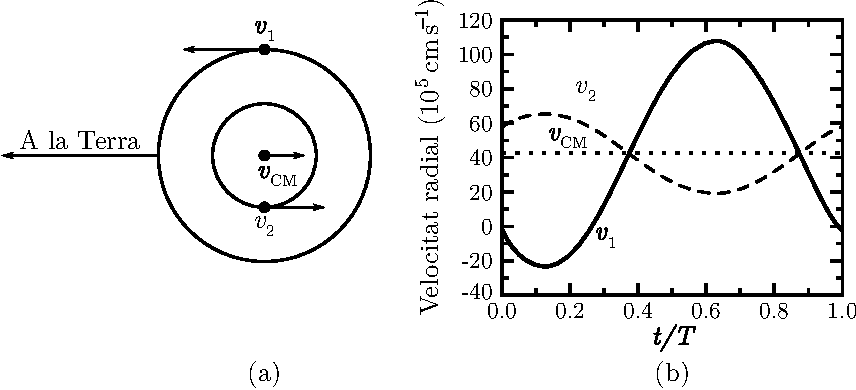
\includegraphics[width=0.8\textwidth]{./images/5-bin-spect-sinus}
	\caption{(a) Dues òrbites circulars el pla de les quals conté la visual de l'observador, (b) corbes de les velocitats radials observades d'ambdues estrelles i del $CM$}
	\label{fig:bin-spect-sinus}
\end{figure}

\begin{itemize}
	\item Si $i \neq \SI{\pi/2}{\radian}$ (la visual ja no pertany al pla de les òrbites) les amplituds queden multiplicades per un factor $\sin i$, però la forma de les corbes no canvia.
	\item Si les òrbites no són circulars (excentricitat $e \neq 0$), les corbes de velocitat observades resultes inclinades (figura \ref{fig:bin-spect-eneq0}) i la forma d'aquestes depèn de l'angle $i$.
\end{itemize}
\begin{figure}[h]
	\centering
	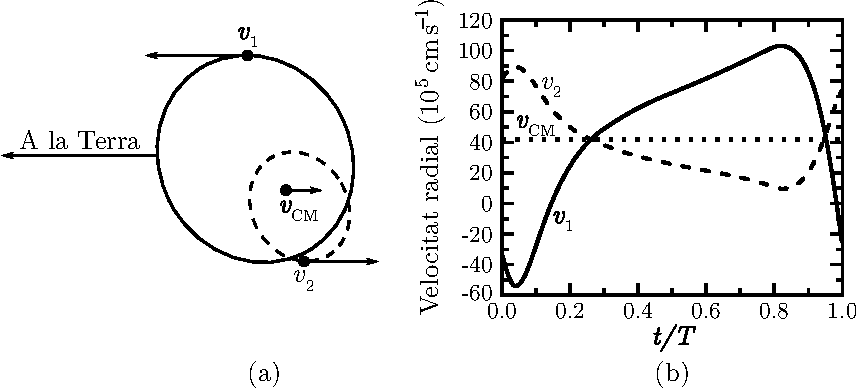
\includegraphics[width=0.8\textwidth]{./images/5-bin-spect-eneq0}
	\caption{Velocitats radials observades. En aquest cas $m_{1} = \SI{0.5}{\Msun}$, $m_{2} = \SI{2.0}{\Msun}$, $a = \SI{2}{\au}$, $e = 0.3$, $i = \SI{\pi/6}{\radian}$}
	\label{fig:bin-spect-eneq0}
\end{figure}

Ja que en realitat moltes binàries posseeixen òrbites de baixa excentricitat suposarem òrbites circulars:
\begin{align*}
	v_{i} = \frac{2\pi a_{i}}{T}
\end{align*}
Utilitzant l'equació \eqref{eq:bin-ma} se segueix
\begin{align}\label{eq:bin-mmvv}
	\frac{m_{1}}{m_{2}} = \frac{v_{2}}{v_{1}}
\end{align}
A més a més, $v_{1 r} = v_{1} \sin i$ i $v_{2 r} = v_{2} \sin i$, de manera que
\begin{align}\label{eq:bin-mmvrvr}
	\frac{m_{1}}{m_{2}} = \frac{v_{2 r}}{v_{1 r}}
\end{align}
Així doncs, el quocient entre ambdues velocitats radials observades ens dóna el quocient entre les masses.

Per determinar la suma de les masses utilitzem l'equació \eqref{eq:bin-mkepler} (Kepler), de manera que
\begin{align}\label{eq:bin-mkepler2}
	m_{1} + m_{2} = \frac{T}{2\pi G} \frac{(v_{1 r} + v_{2 r})^{3}}{\sin^{3} i}
\end{align}
Així doncs, hem de conèixer les components radials de la velocitat d'ambdues estrelles.

Amb freqüència una estrella (e.g., la 1) és molt més brillant que l'altra, de forma que l'espectre d'aquesta resulta inaccessible. En aquest cas només es coneix $v_{1 r}$ i no és possible determinar les masses individuals. No obstant, utilitzant la relació \eqref{eq:bin-mmvrvr} per eliminar $v_{2 r}$ de l'equació \eqref{eq:bin-mkepler2}, tenim:
\begin{align*}
	m_{1} + m_{2} = \frac{T}{2\pi G} \frac{v_{1 r}^{3}}{\sin^{3} i} \qty(1 + \frac{m_{1}}{m_{2}})^{3}
\end{align*}
i després de reordenar els termes obtenim
\begin{align}\label{eq:bin-mkepler3}
	\frac{m_{2}^{3}}{(m_{1} + m_{2})^{2}} \sin^{3} i = \frac{T}{2\pi G} v_{1 r}^{3}
\end{align}

El costat dret de l'expressió \eqref{eq:bin-mkepler3} es coneix com la \textit{funció de massa}, i depèn només de les magnituds obtingudes mitjançant l'observació (període i velocitat radial de l'estrella 1).
\begin{figure}[h]
	\centering
	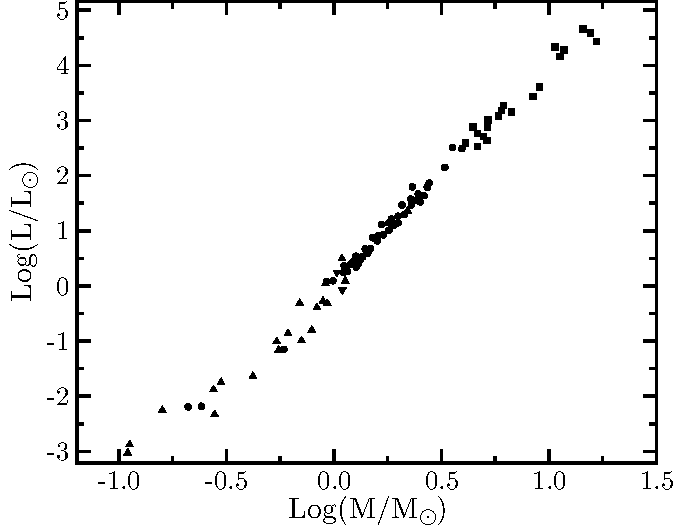
\includegraphics[width=0.6\textwidth]{./images/5-bin-spect-m-l}
	\caption{Relació massa--lluminositat. ($\bullet$) Sistemes de la seqüència principal distants, B6 fins M, ($\blacktriangle$) binàries visuals, (${\scriptstyle \blacksquare}$) sistemes OB distants, ($\blacktriangledown$) binàries espectroscòpiques resoltes}
	\label{fig:bin-spect-m-l}
\end{figure}

Ja que no és es coneix l'espectre de l'estrella 1, no és possible determinar $m_{1} / m_{2}$. En conseqüència, la funció de massa és útil només per a estudis estadístics o si una estimació de la massa d'un dels components fos possible per mètodes indirectes.

Si $m_{1}$ o bé $\sin i$ fos desconegut, la funció de massa imposa un límit sobre $m_{2}$, ja que el costat esquerre de l'equació \eqref{eq:bin-mkepler3} és inferior a $m_{2}$.

Gràcies a la determinació de masses en sistemes binaris s'ha aconseguit obtenir una relació empírica massa--lluminositat per a la majoria de les estrelles del firmament (figura \ref{fig:bin-spect-m-l}).

%-----------------------------
\subsubsection*{Determinació de les masses d'un sistema espectroscòpic binari eclipsant}
Si el sistema espectroscòpic binari és a més eclipsant, es pot obtenir informació addicional.
\begin{figure}[H]
	\centering
	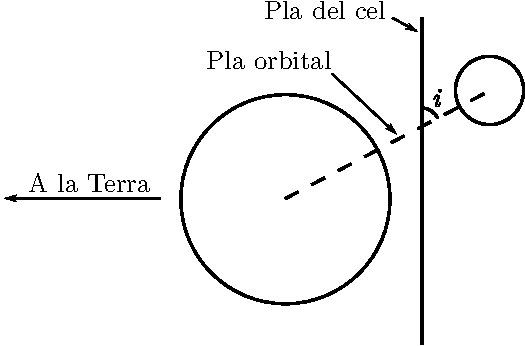
\includegraphics[width=0.5\textwidth]{./images/5-bin-pi2}
	\caption{Geometria d'una binària espectroscòpica eclipsant requereix que l'angle d'inclinació sigui $i \approx \SI{\pi/2}{\radian}$}
	\label{fig:bin-pi2}
\end{figure}

En primer lloc, l'angle $i$ entre el pla de les òrbites i el pla cel cel ha de ser pròxim a $\SI{\pi/2}{\radian}$ (figura \ref{fig:bin-pi2}).

La duració dels eclipsis permet estimar els radis d'ambdues estrelles. Per simplificar\footnote{Cal notar, que en el desenvolupament hem menyspreat l'efecte dels llimbs i la possible no esfericitat de les estrelles a causa de la presència de l'altra.} el desenvolupament, suposem que $i \equiv \SI{\pi/2}{\radian}$.
\begin{figure}[h]
	\centering
	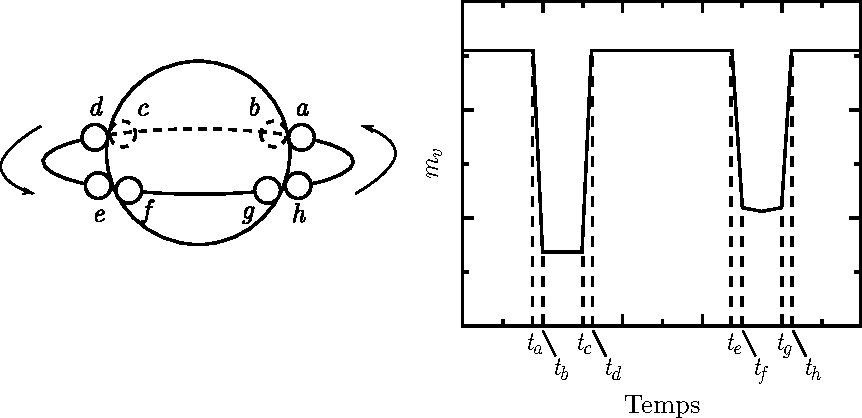
\includegraphics[width=0.8\textwidth]{./images/5-bin-eclipses}
	\caption{Corba de llum d'una binària eclipsant amb $i = \SI{\pi/2}{\radian}$. Els temps indicats en l'eix de les abscisses corresponen a les posicions successives de l'estrella petita respecte a la gran. Entre $t_{b}$ i $t_{c}$ la petita es troba totalment oculta per la gran. Aquí se suposa implícitament que la petita és de major temperatura que la gran}
	\label{fig:bin-eclipses}
\end{figure}

De la figura \ref{fig:bin-eclipses}, deduïm que el radi de l'estrella petita és donat aproximadament per
\begin{align}
	r_{s} = \frac{1}{2} v (t_{b} - t_{a})
\end{align}
i deduïm que el radi de l'estrella gran és aproximadament
\begin{align}
	r_{l} = \frac{1}{2} v (t_{c} - t_{a})
\end{align}
on $v = v_{s} + v_{l}$ és la velocitat relativa d'ambdues estrelles.

El flux de radiació en la superfície (de cada estrella) ve donat per
\begin{align}\label{eq:F-T}
   F = \sigma T_{e}^{4}
\end{align}

Suposem que l'estrella de major temperatura és la petita. Referint-nos de nou a la figura \ref{fig:bin-eclipses}, la brillantor quan ambdues estrelles són totalment visibles és
\begin{align}
	B_{0} = k (\pi r_{l}^{2} F_{l} + \pi r_{s}^{2} F_{s}) \qc (k > 0)
\end{align}
En el primer mínim (el més profund $\Rightarrow$ estrella petita oculta) la brillantor serà
\begin{align*}
	B_{p} = k \pi r_{l}^{2} F_{l}
\end{align*}
En el segon mínim (estrella gran parcialment oculta), la brillantor serà
\begin{align*}
	B_{s} = k (\pi r_{l}^{2} - \pi r_{s}^{2}) F_{l} + k \pi r_{s}^{2} F_{s}
\end{align*}
Com que la constant $k$ no es pot determinar amb prou exactitud hem de conformar-nos amb el quocient
\begin{align*}
	\frac{B_{0} - B_{p}}{B_{0} - B_{s}} = \frac{F_{s}}{F_{l}}
\end{align*}
i utilitzant l'equació \eqref{eq:F-T}, obtenim
\begin{align}
	\frac{B_{0} - B_{p}}{B_{0} - B_{s}} = \qty(\frac{T_{s}}{T_{l}})^{4}
\end{align}
